\documentclass[12pt, a4paper]{ctexart}

\usepackage{fancyhdr}
\pagestyle{fancy}
\fancyhead{}
\renewcommand{\headrulewidth}{1pt}
\renewcommand{\headwidth}{\textwidth}
\fancyhead[L]{\leftmark}
\fancyhead[R]{\thepage}
\fancyfoot{}

\fancypagestyle{plain}{
\fancyhead{}
\renewcommand{\headrulewidth}{1pt}
\fancyfoot{}
\fancyhead[L]{北京大学基础物理实验报告}
\fancyhead[R]{唐晨宇}
}
\usepackage[colorlinks,linkcolor=red,urlcolor = blue]{hyperref}
\usepackage{booktabs}
\usepackage{graphicx}
\usepackage{amsmath}
\usepackage{mathcomp}
\usepackage{mathabx}
\usepackage{enumitem}
\usepackage[top=1.2in, bottom=1.2in, left=1in, right=1in]{geometry}
\usepackage{subfig}

\ctexset{
    section={   
        name={,},
        number={\chinese{section}},
        format=\heiti\raggedright
    },
    subsection={   
        name={(,)},
        number={\chinese{subsection}},
        format=\heiti
    }
}

\begin{document}
\title{RLC电路的谐振现象}
\author{唐晨宇 \quad 2300934207}
\date{2024年4月}

\maketitle
\tableofcontents
\clearpage


\section*{实验仪器}
DG1022U函数/任意波形发生器,TFG6920A信号源,SS7802A模拟示波器,TBS\;1202B-EDU数字示波器,台式万用表,RX7-0型十进位电容器,100$\Omega$标准电阻,BG6-4\;0.1H标准电感箱

\section{谐振频率测量}
\subsection{利用数字万用表测量谐振电阻分压}
信号源输出波形幅值$U_{ppR} = 1.000 V$,当输出频率为$2.2507 kHz$时,标准电阻上的分压达到最大值,测得$U_{Rmax} = 205.00mV$.

在调节过程中在谐振频率上下$0.1Hz$范围内电阻分压幅值无明显差别,故可认为测量误差为$\sigma_{f_0} = 0.1Hz$,即谐振频率$f_0 \pm \sigma_{f_0} = (2250.7 \pm 0.1)Hz$.

\subsection{利用模拟示波器测量谐振电阻分压}
输出条件同上,测量结果与数字万用表没有明显差别,不再重复.

\subsection{利用李萨如图判断电压电流相位差零点}
输出条件同上,当输出频率为$2.2487 kHz$时,交流电路中电流与电压形成的李萨如图呈直线,即相差为0.

\subsection{电路参数计算谐振频率}
当前电路中各参数如下:
\begin{description}
    \item[电容] 电容器允差$e_C = 0.5\%C$,算得$C \pm \sigma_{C} = (0.05000 \pm 0.00015) \mu F$.
    \item[电感] 标准自感允差$e_L= 0.1\%L$,算得$L \pm \sigma_{L} = (0.10000 \pm 0.00006) H$.
\end{description}

对于RLC谐振电路,谐振频率为$f_0 = \frac{1}{2\pi \sqrt{LC}} = 2251 Hz$,不确定度
\begin{equation*}
    \sigma_{f_0} = \sqrt{(\frac{\partial f_0}{\partial C})^2 \sigma_C^2 + (\frac{\partial f_0}{\partial L})^2 \sigma_L^2} = \frac{f_0}{2} \sqrt{(\frac{\sigma_C}{C})^2 + (\frac{\sigma_L}{L})^2} = 4Hz
\end{equation*}
故谐振频率$f_0 \pm \sigma_{f_0} = (2251 \pm 4) Hz$,上述测量结果均在误差范围内.

\section{相频曲线测量}
数据见表\ref{tab:t1},相应图像如图\ref{fig1}\\
\begin{table}[htbp]
  \centering
  \caption{频率-相位差数据表}
    \begin{tabular}{c|ccccccc}
    \toprule
    $f/kHz$      & 2.000 & 2.040 & 2.080 & 2.120 & 2.160 & 2.170 & 2.180 \\
    $\Delta t/ms$& 0.1540 & 0.1560 & 0.1590 & 0.1650 & 0.1780 & 0.1800 & 0.1850 \\
    $\Delta \phi /\pi$ & -0.38400 & -0.36352 & -0.33856 & -0.30040 & -0.23104 & -0.21880& -0.19340 \\
    \midrule
    $f/kHz$      & 2.190 & 2.200 & 2.210 & 2.220 & 2.230 & 2.240 & 2.242 \\
    $\Delta t/ms$& 0.1890 & 0.1940 & 0.2000 & 0.2050 & 0.2110 & 0.2165 & 0.2180\\
    $\Delta \phi /\pi$ & -0.17218& -0.14640& -0.11600& -0.08980& -0.05894 & -0.03008 & -0.02249 \\
    \midrule
    $f/kHz$      & 2.244 & 2.246 & 2.248 & 2.250 & 2.260 & 2.270 & 2.280 \\ 
    $\Delta t/ms$& 0.2195 & 0.2225 & 0.2225 & 0.2230 & 0.2295 & 0.2355 & 0.2405 \\
    $\Delta \phi /\pi$ & -0.01488 & -0.00053 & 0.00036 & 0.00350 & 0.03734 & 0.06917 & 0.09668 \\
    \midrule
    $f/kHz$      & 2.290 & 2.300 & 2.310 & 2.320 & 2.330 & 2.340 & 2.350 \\
    $\Delta t/ms$& 0.2460 & 0.2505 & 0.2545 & 0.2580 & 0.2615 & 0.2640 & 0.2670 \\
    $\Delta \phi /\pi$ & 0.12668 & 0.15230 & 0.17579 & 0.19712 & 0.21859 & 0.23552 & 0.25490 \\
    \midrule
    $f/kHz$      & 2.360 & 2.370 & 2.380 & 2.390 & 2.400 & 2.500 & 2.600 \\
    $\Delta t/ms$& 0.2680 & 0.2705 & 0.2710 & 0.2730 & 0.2735 & 0.2755 & 0.2710 \\
    $\Delta \phi /\pi$ & 0.26496 & 0.28217 & 0.28996 & 0.30494 & 0.3128 & 0.3775 & 0.4092 \\
    \bottomrule
    \end{tabular}
  \label{tab:t1}
\end{table}
其中$\Delta \phi = 2\pi \frac{\Delta t}{T} = 2\pi \Delta tf$.
\begin{figure}
    \centering
    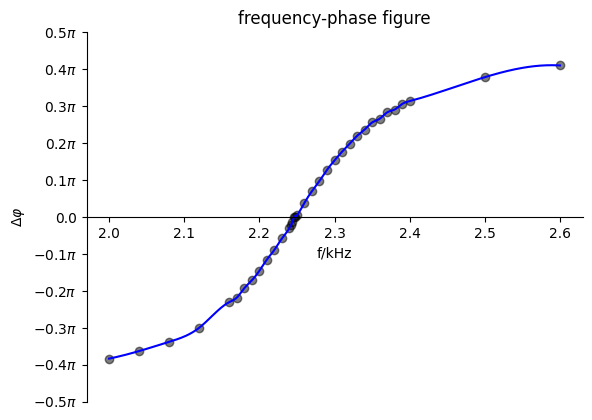
\includegraphics[width = 4in]{figure/frequency-phase figure.png}
    \caption{相频特性曲线(部分)}
    \label{fig1}
\end{figure}

从图中可以看出,电流电压同相时输入交流电压频率约为$2249Hz$,与前述测量结果基本相符。

\section{幅频曲线测量及$Q$值的第三种意义}
数据见表\ref{tab:t2},相应图像如图\ref{fig2}
\begin{table}[htbp]
  \centering
  \caption{频率-电流幅值数据表}
    \begin{tabular}{c|ccccccc}
    \toprule
    $f/kHz$ & 0.500  & 0.700 & 0.900 & 1.100 & 1.300 & 1.500 & 1.700 \\
    $i / \times 10^{-2} mA$ & 5.89 & 8.65 & 11.93 & 16.06 & 21.60 & 29.72 & 43.07 \\
    \midrule
    $f/kHz$ & 2.000  & 2.010 & 2.020 & 2.030 & 2.040 & 2.050 & 2.060 \\
    $i / \times 10^{-2} mA$ & 94.12 & 97.37 & 100.81 & 104.43 & 108.25 & 112.28 & 116.54 \\
    \midrule
    $f/kHz$ & 2.070 & 2.080 & 2.090 & 2.100 & 2.110 & 2.120 & 2.130 \\
    $i / \times 10^{-2} mA$ & 121.01 & 125.72 & 130.68 & 135.86 & 141.25 & 146.85 & 152.63\\
    \midrule
    $f/kHz$ & 2.140 & 2.150 & 2.160 & 2.170 & 2.180 & 2.190 & 2.200 \\
    $i / \times 10^{-2} mA$ & 158.54 & 164.54 & 170.55 & 176.47 & 182.20 & 187.59 & 192.50 \\
    \midrule
    $f/kHz$ & 2.210 & 2.220 & 2.230 & 2.240 & 2.242 & 2.244 & 2.246 \\
    $i / \times 10^{-2} mA$ & 196.77 & 200.25 & 202.82 & 204.36 & 204.54 & 204.68 & 204.77 \\
    \midrule
    $f/kHz$ & 2.248 & 2.250 & 2.252 & 2.254 & 2.256 & 2.258 & 2.260 \\
    $i / \times 10^{-2} mA$ & 204.82 & 204.82 & 204.79 & 204.70 & 204.58 & 204.41 & 204.20 \\
    \midrule
    $f/kHz$ & 2.270 & 2.280 & 2.290 & 2.300 & 2.310 & 2.320 & 2.330 \\
    $i / \times 10^{-2} mA$ & 202.53 & 199.91 & 196.48 & 192.27 & 187.64 & 182.56 & 177.22 \\
    \midrule
    $f/kHz$ & 2.340 & 2.350 & 2.360 & 2.370 & 2.380 & 2.390 & 2.400 \\
    $i / \times 10^{-2} mA$ & 171.73 & 166.20 & 160.73 & 155.31 & 150.06 & 144.97 & 140.07 \\
    \midrule
    $f/kHz$ & 2.600 & 2.800 & 3.000 & 3.200 & 3.400 & 3.600 & 3.800 \\
    $i / \times 10^{-2} mA$ & 79.18 & 54.42 & 41.74 & 34.08 & 28.94 & 29.25 & 22.47 \\
    \midrule
    $f/kHz$ & 4.000 & 4.200 & 4.400 & 4.600 & 4.800 &   &   \\
    $i / \times 10^{-2} mA$ & 20.28 & 18.52 & 17.06 & 15.84 & 14.79 &   &   \\
    \bottomrule
    \end{tabular}
  \label{tab:t2}
\end{table}

\begin{figure}
    \centering
    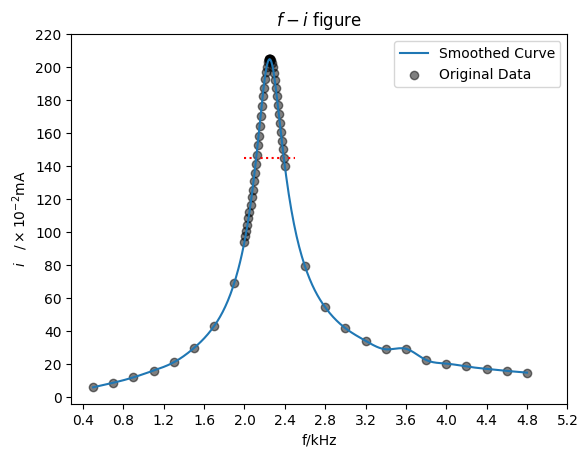
\includegraphics[width = 4in]{figure/f-i figure.png}
    \caption{幅频特性曲线(部分)}
    \label{fig2}
\end{figure}
其中测量值为电阻分压有效值,$i = \frac{U_{Reff}}{R}$.

从图中可以看出,电流有效值峰值约为$2.0482mA$,在输入频率为$2.253kHz$附近出现.
而相应半值宽度$\frac{i_{max}}{\sqrt{2}} = 1.4483Hz$,即图中红线对应值则分别在$f_1 = 2.1164kHz$和$2.3903kHz$处出现.
故由$Q$值的第三种意义可得$Q_3 = \frac{f_0}{\Delta f} = 8.226$

我们可以认为谐振频率的不确定度$\sigma_{f_0} = 1Hz$,而半值宽度的不确定度$\sigma_{\Delta f} = 0.1Hz$,故
\begin{equation*}
  \sigma_{Q_3} = Q_3\sqrt{(\frac{\sigma_{f_0}}{f_0})^2 + (\frac{\sigma_{\Delta f}}{\Delta f})^2} = 0.005
\end{equation*}
即最终结果为$Q_3 \pm \sigma_{Q_3} = 8.226 \pm 0.005$\footnotemark.
\footnotetext{本实验报告中各处数据及模型的研究对象均为包括了示波器内阻的交流电压源之外的整体外电路,包括标注电阻、示波器电容电感内阻、各种耗散产生的等效电阻及标准电容和标准电感,
因此各处结论(尤其是关于$Q$值的计算)会与标准值存在偏差,但相对于该实验报告是自洽的.}

\section{$Q$值的第一种意义}
谐振时电容与电感阻抗之和为零,因此电路中总电阻可用谐振时电压值除以电流值算得.

利用示波器测得$(100.00 \pm 0.01)\Omega$标准电阻分压$U_{ppR} = 1.518V$,信号源输出电压$U_{ppinput} = 2.500V$,故
\begin{equation*}
  R_{tot} = \frac{U_{ppinput}}{U_{ppR}}R = 164.7\Omega
\end{equation*}
数字万用表交流电压档允差为$0.2\% + 10$个字,相应算得$e_{U_{ppR}} = 0.005V$.
同时可以认为$\sigma_{U_{ppinput}} = 0.001V$,故
\begin{equation*}
  \sigma_{R_{tot}} = R_{tot}\sqrt{(\frac{\sigma_{U_{ppinput}}}{U_{ppinput}})^2 + (\frac{e_{U_{ppR}}/\sqrt{3}}{U_{ppR}})^2 + (\frac{\sigma_{R}}{R})^2} = 0.4\Omega
\end{equation*}
算得
\begin{gather*}
  Q_1 = \frac{\omega_0 L}{R_{tot}} = \frac{1}{R \omega_0 C} = \frac{1}{R}\sqrt{\frac{L}{C}} = 8.587\\
  \sigma_{Q_1} = Q_1\sqrt{(\frac{1}{2}\frac{\sigma_L}{L})^2 + (\frac{1}{2}\frac{\sigma_C}{C})^2 + (\frac{\sigma_R}{R})^2} = 0.025
\end{gather*}
故最终结果为$Q_1 \pm \sigma_{Q_1} = 8.587 \pm 0.025$

\section{$Q$值的第二种意义}
$Q$值也可表征串联谐振电路电压放大的特性,利用数字万用表测量得谐振时$u_L = 2.8470V$,$u_C = 2.8385V$,信号源输出电压$U_{ppinput} = 1.000V$,故$Q_2 = \frac{\bar{u}}{U_{ppinput}/2\sqrt{2}} = 8.040$.
相应不确定度$\sigma_{\bar{u}} = \frac{u}{\sqrt{3}} = 0.004V$,$\sigma_{U_{ppinput}} = 0.001V$,算得$\sigma_{Q_2} = Q_2\sqrt{(\frac{\sigma_{\bar{u}}}{\bar{u}})^2 + (\frac{\sigma_{U_{ppinput}}}{U_{ppinput}})^2} = 0.014$.
故最终结果为$Q_2 + \sigma_{Q_2} = 8.040 \pm 0.014$.

\section{拓展实验:选频滤波}
\subsection{非简谐信号的快速傅里叶变换}
在RLC电路上加上频率为$1kHz$的$1:1$方波输入电压,利用数字示波器测量电阻分压,可以得到振荡衰减的波形.
利用数字示波器的快速傅里叶变换功能可以得到如图\ref{fig3}频域波形.
\begin{figure}[htbp]
  \centering
  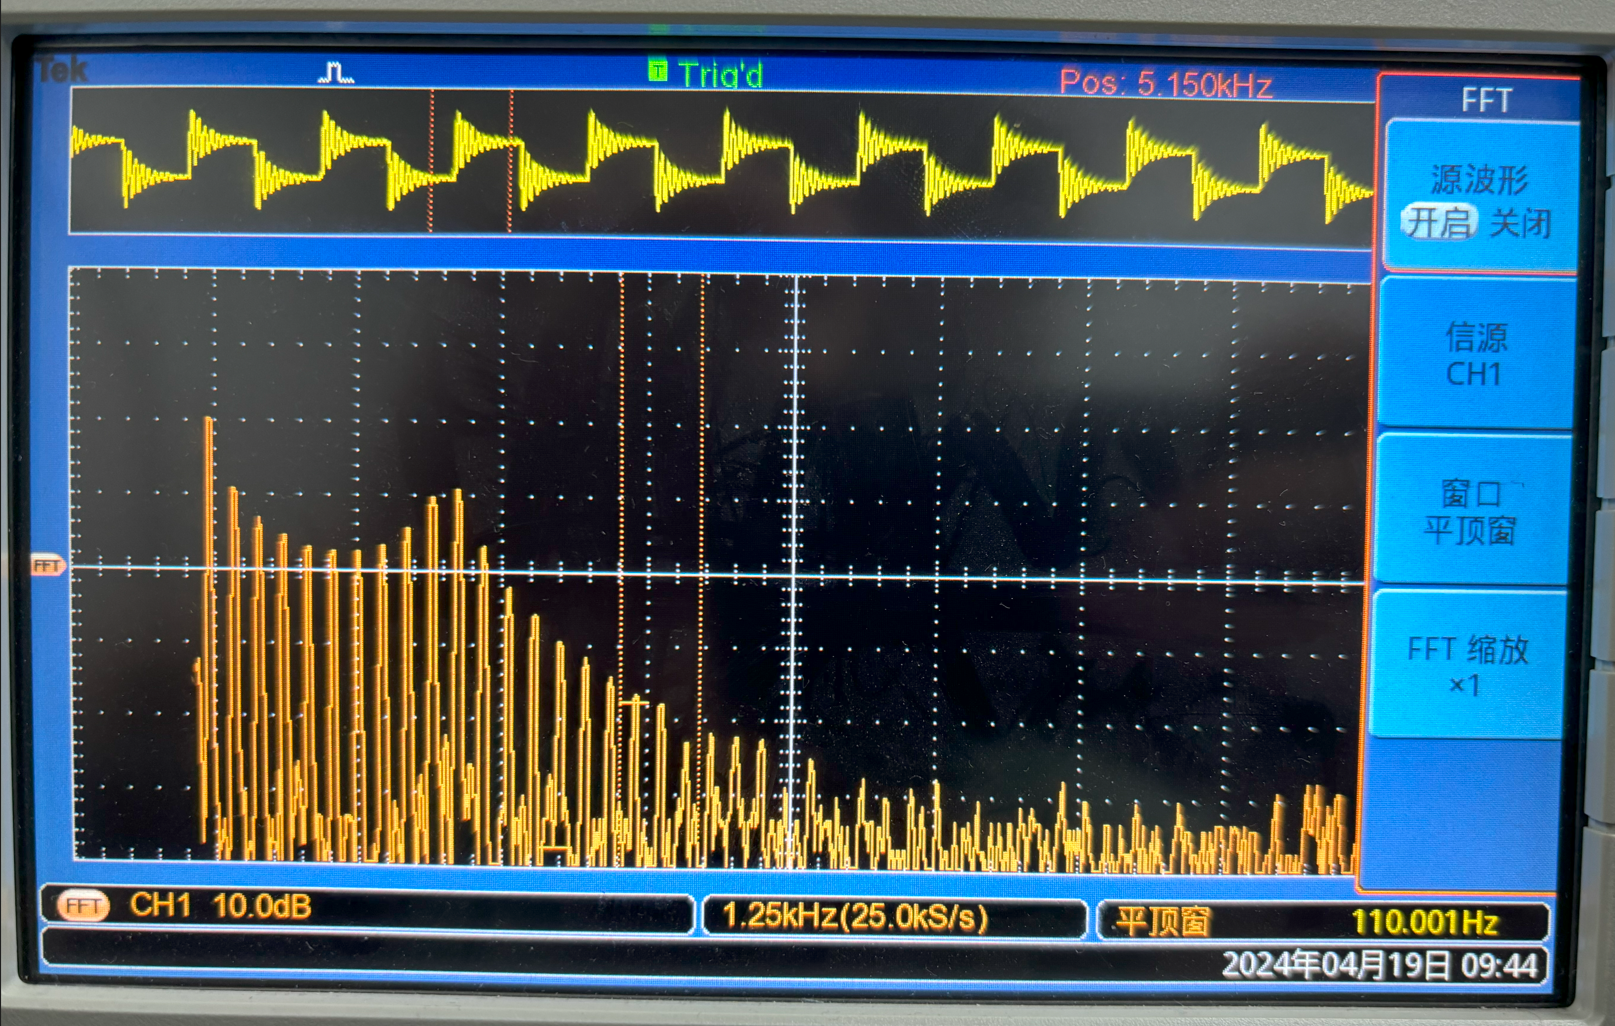
\includegraphics[width = 4in]{figure/FFT.png}
  \caption{}
  \label{fig3}
\end{figure}

利用光标测量得出,该振荡波形中包含$1kHz, 3kHz, 5kHz$等一系列不同频率的简谐成分,具体计算此处不详细解释.


\subsection{方波信号的选频滤波}
输入信号为频率为$1kHz$的$1:1$方波.

我们知道,某一组电路参数对应的谐振频率在该电路条件下具有最大的振幅,最容易在示波器上显示.
因此我们在控制标准电感大小为$1H$的条件下通过调节电容大小来测量相应谐振频率的成分.\\
对于$1kHz$成分,$\frac{1}{2\pi \sqrt{LC_1}} = 1kHz \Rightarrow C_1 = 0.2533 \mu F$.\\
对于$3kHz$成分,$\frac{1}{2\pi \sqrt{LC_2}} = 3kHz \Rightarrow C_2 = 0.02814 \mu F$,以上同理.

测量得到如图\ref{fig4}结果.
\begin{figure}[htbp]
  \centering
  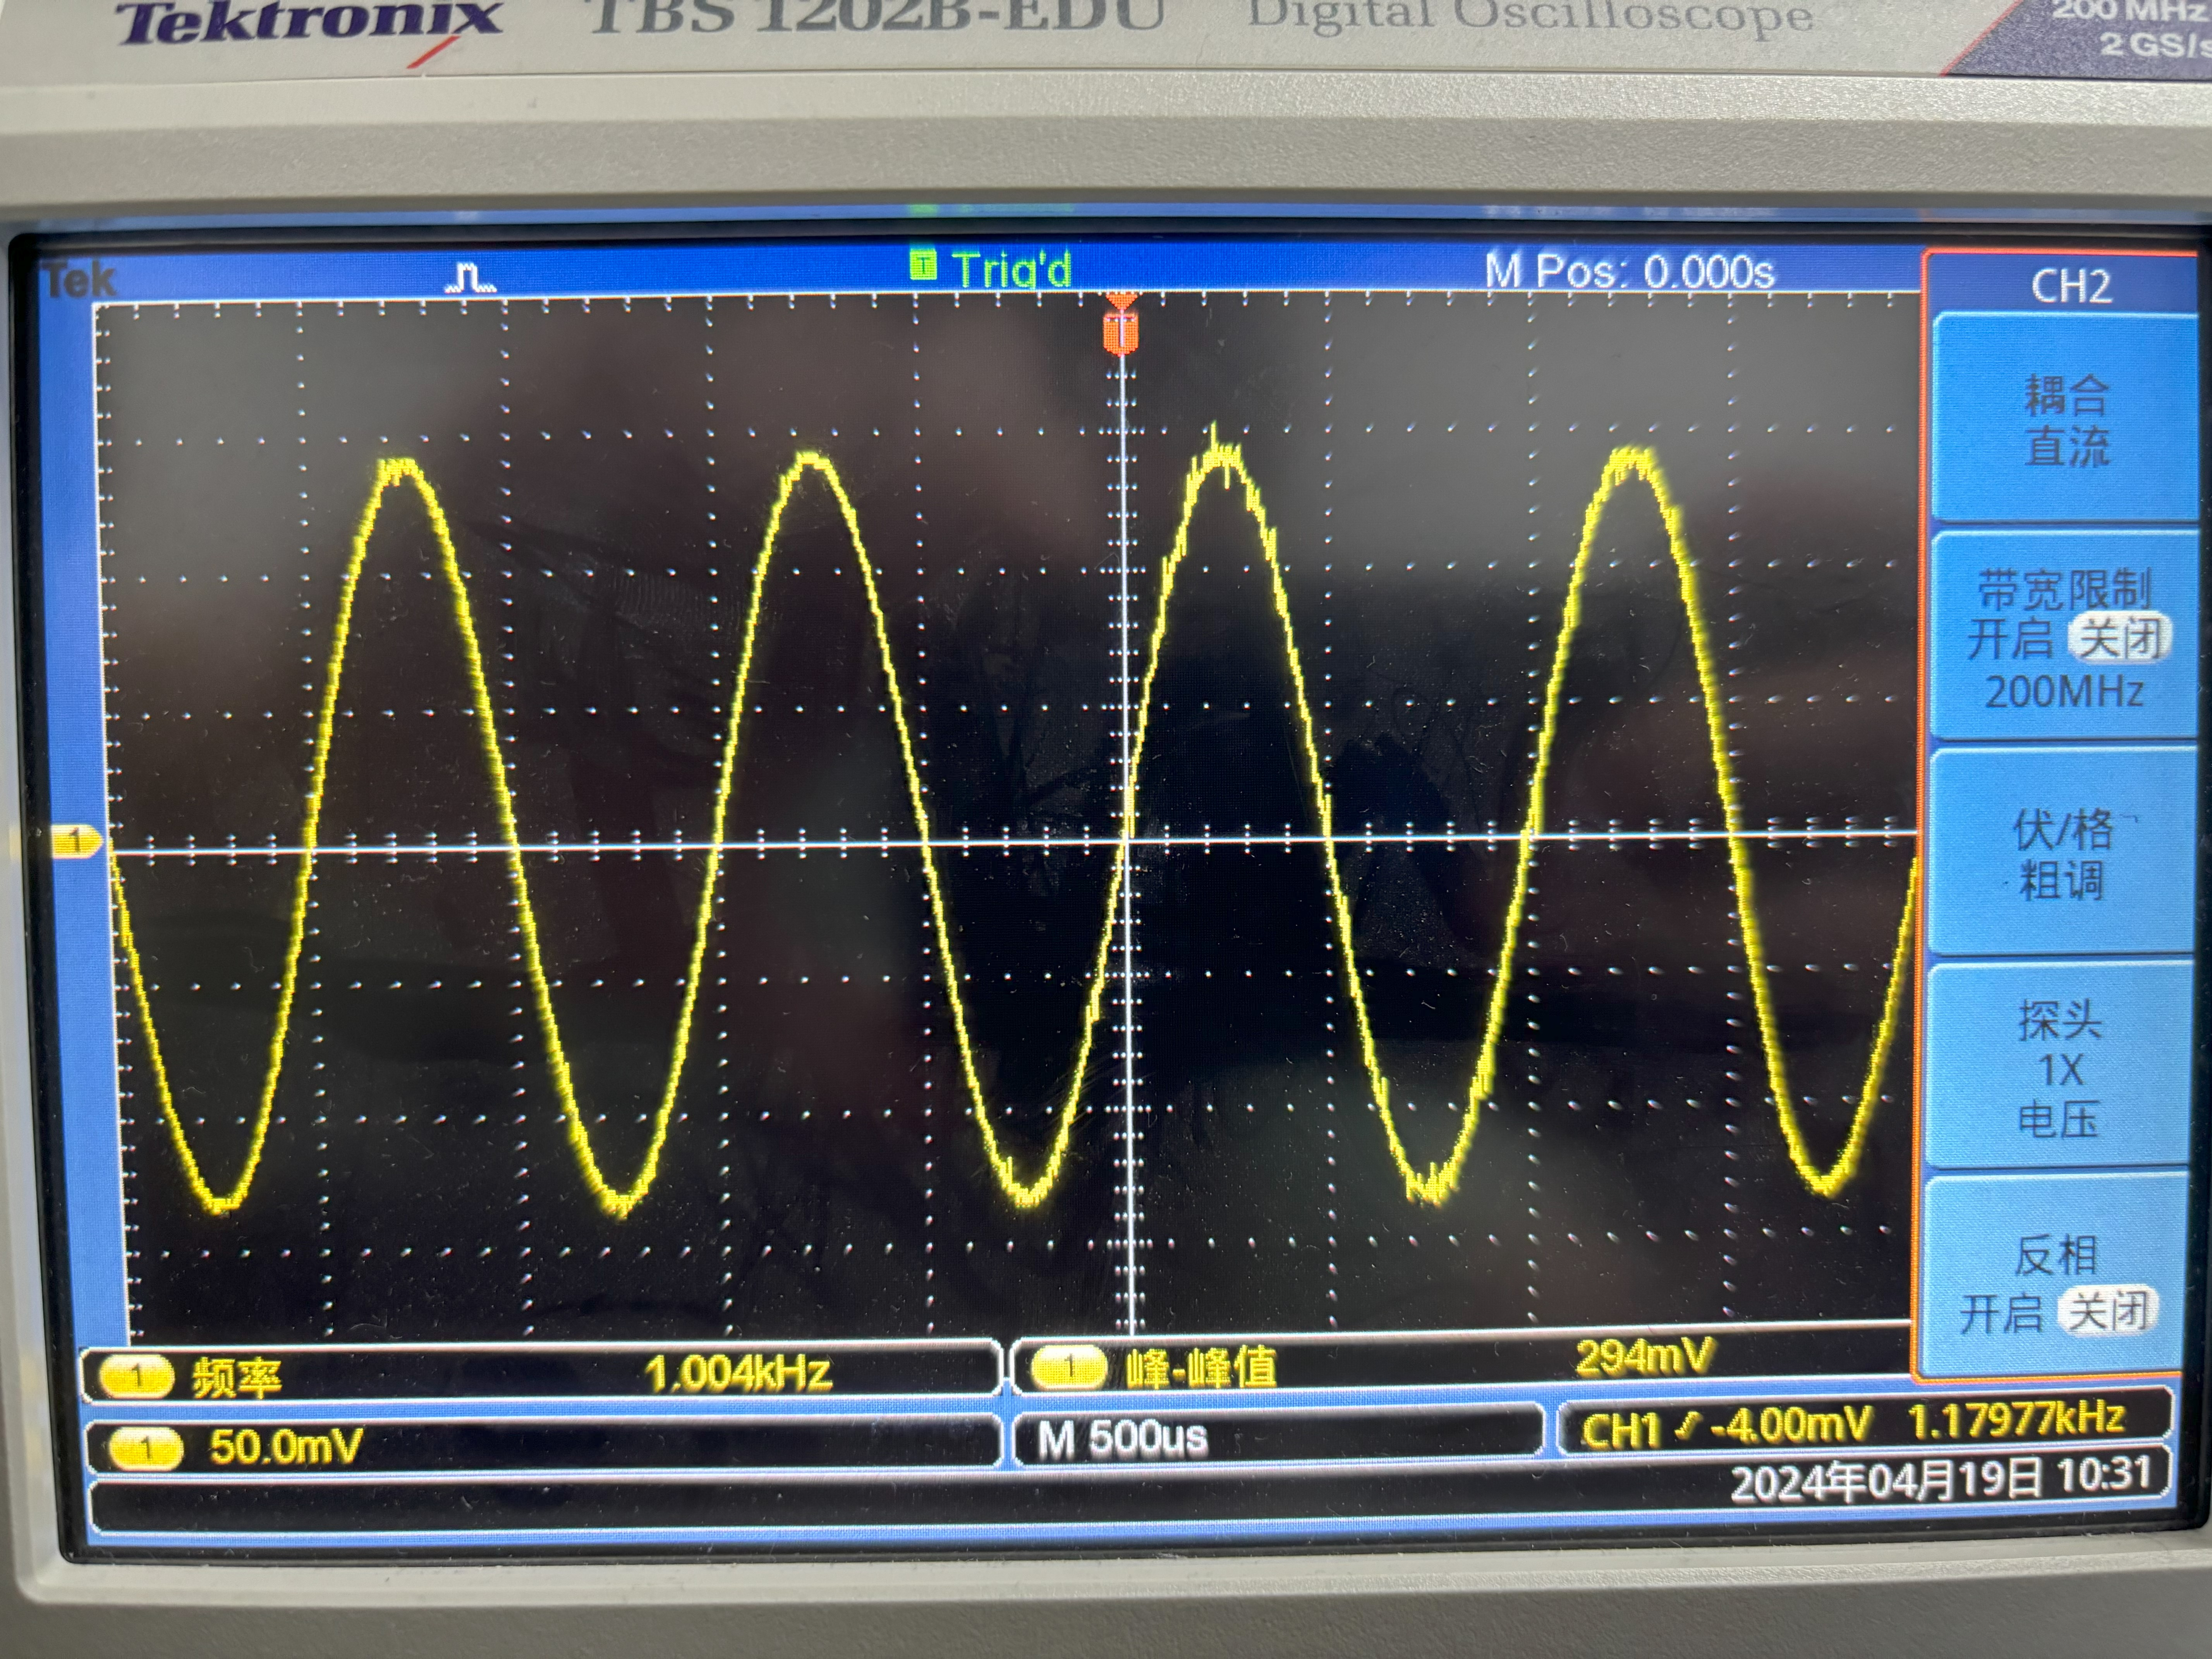
\includegraphics[width = 2in]{figure/1kHz.jpg}
  \includegraphics[width = 2in]{figure/3kHz.jpg}
  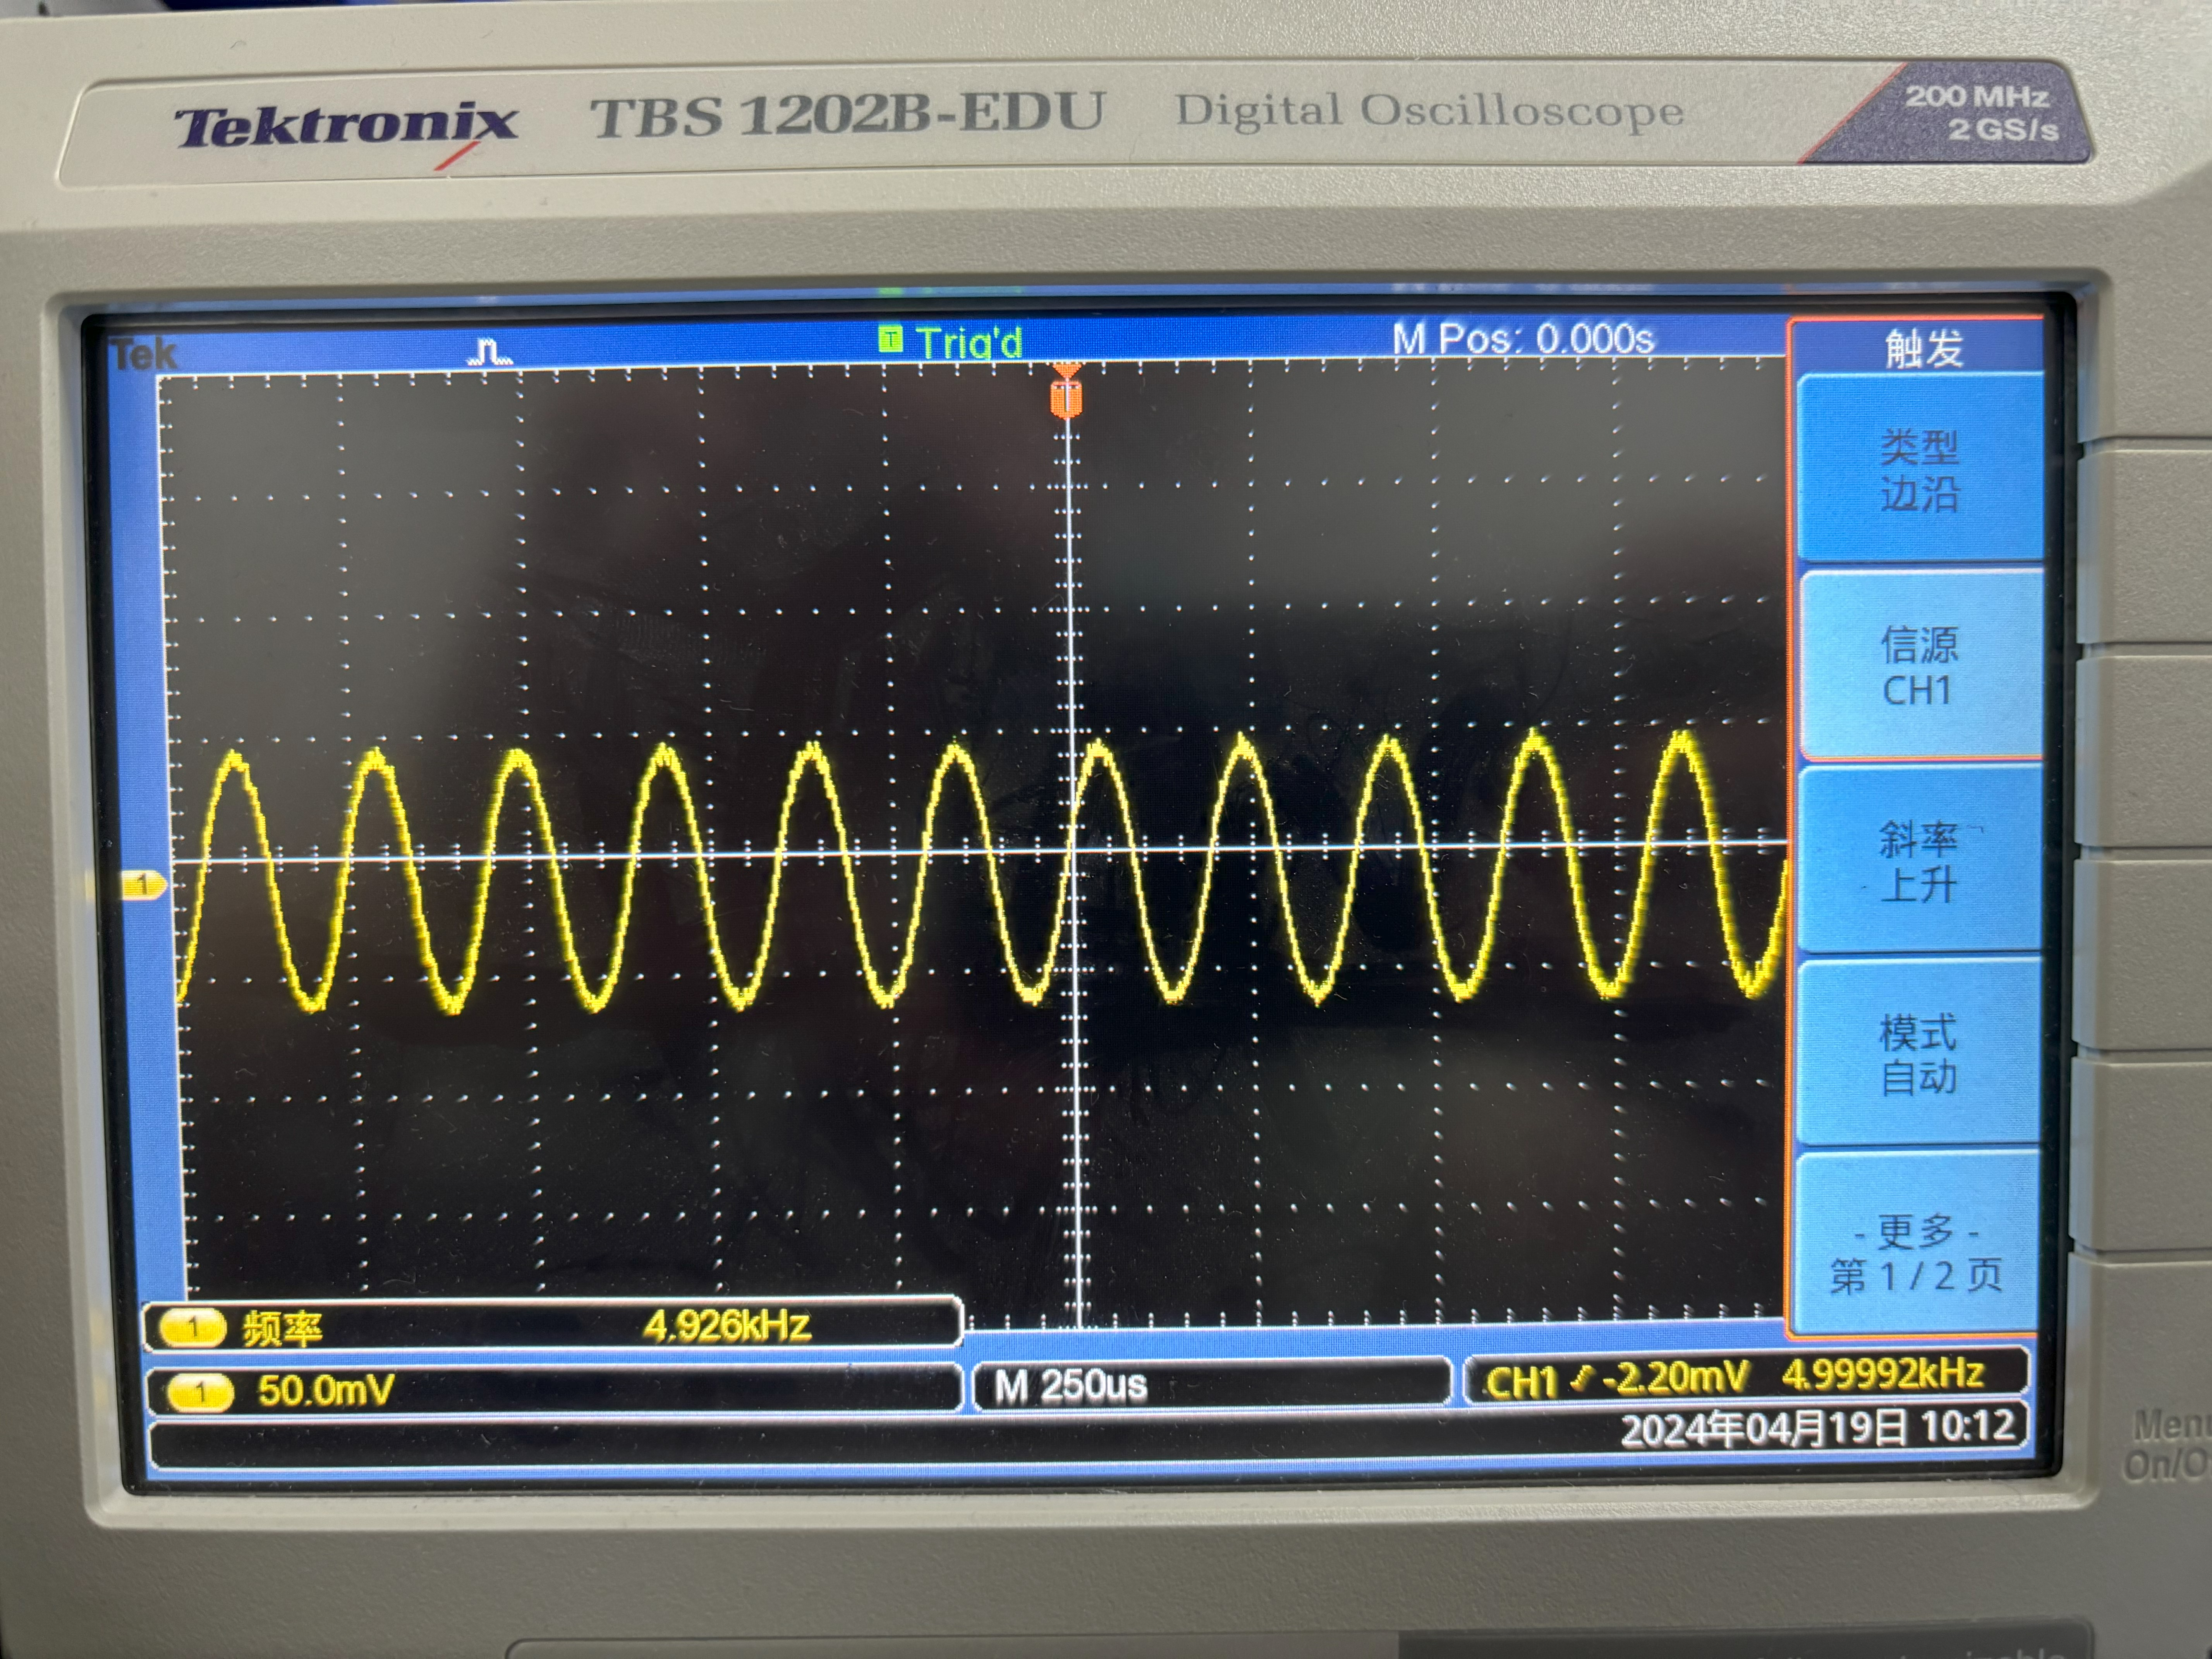
\includegraphics[width = 2in]{figure/5kHz.jpg}
  \caption{}
  \label{fig4}
\end{figure}

从图中可以看出,$1kHz$成分的幅值为约$290mV$,而$3kHz$成分的幅值为约$80mV$,大致为3.6倍关系.

理论推导可以得出,对方波进行傅里叶分解的结果为
\begin{equation*}
  f(t) \sim \frac{4A_{max}}{\pi} \sum_{n=1}^{\infty} \frac{\sin((2n - 1)\omega t)}{2n - 1}
\end{equation*}

可以看到一倍与三倍频的幅值应为三倍关系.
简单分析可以得到,图中一倍频波形稳定平滑,但三倍频的幅值存在波动,波形中也明显存在杂波成分干扰,因此可以猜想是对三倍频进行选频时对高频部分的滤波不够彻底,导致对幅值的测量不准确使幅值倍率偏离理论值.

\subsection{三角波信号的选频滤波}
输入信号为频率为$1kHz$的$1:1$三角波.

一倍频选频结果如图\ref{fig5}所示.
由于水平有限,未能调节出较为稳定的三倍频信号……
\begin{figure}[htbp]
  \centering
  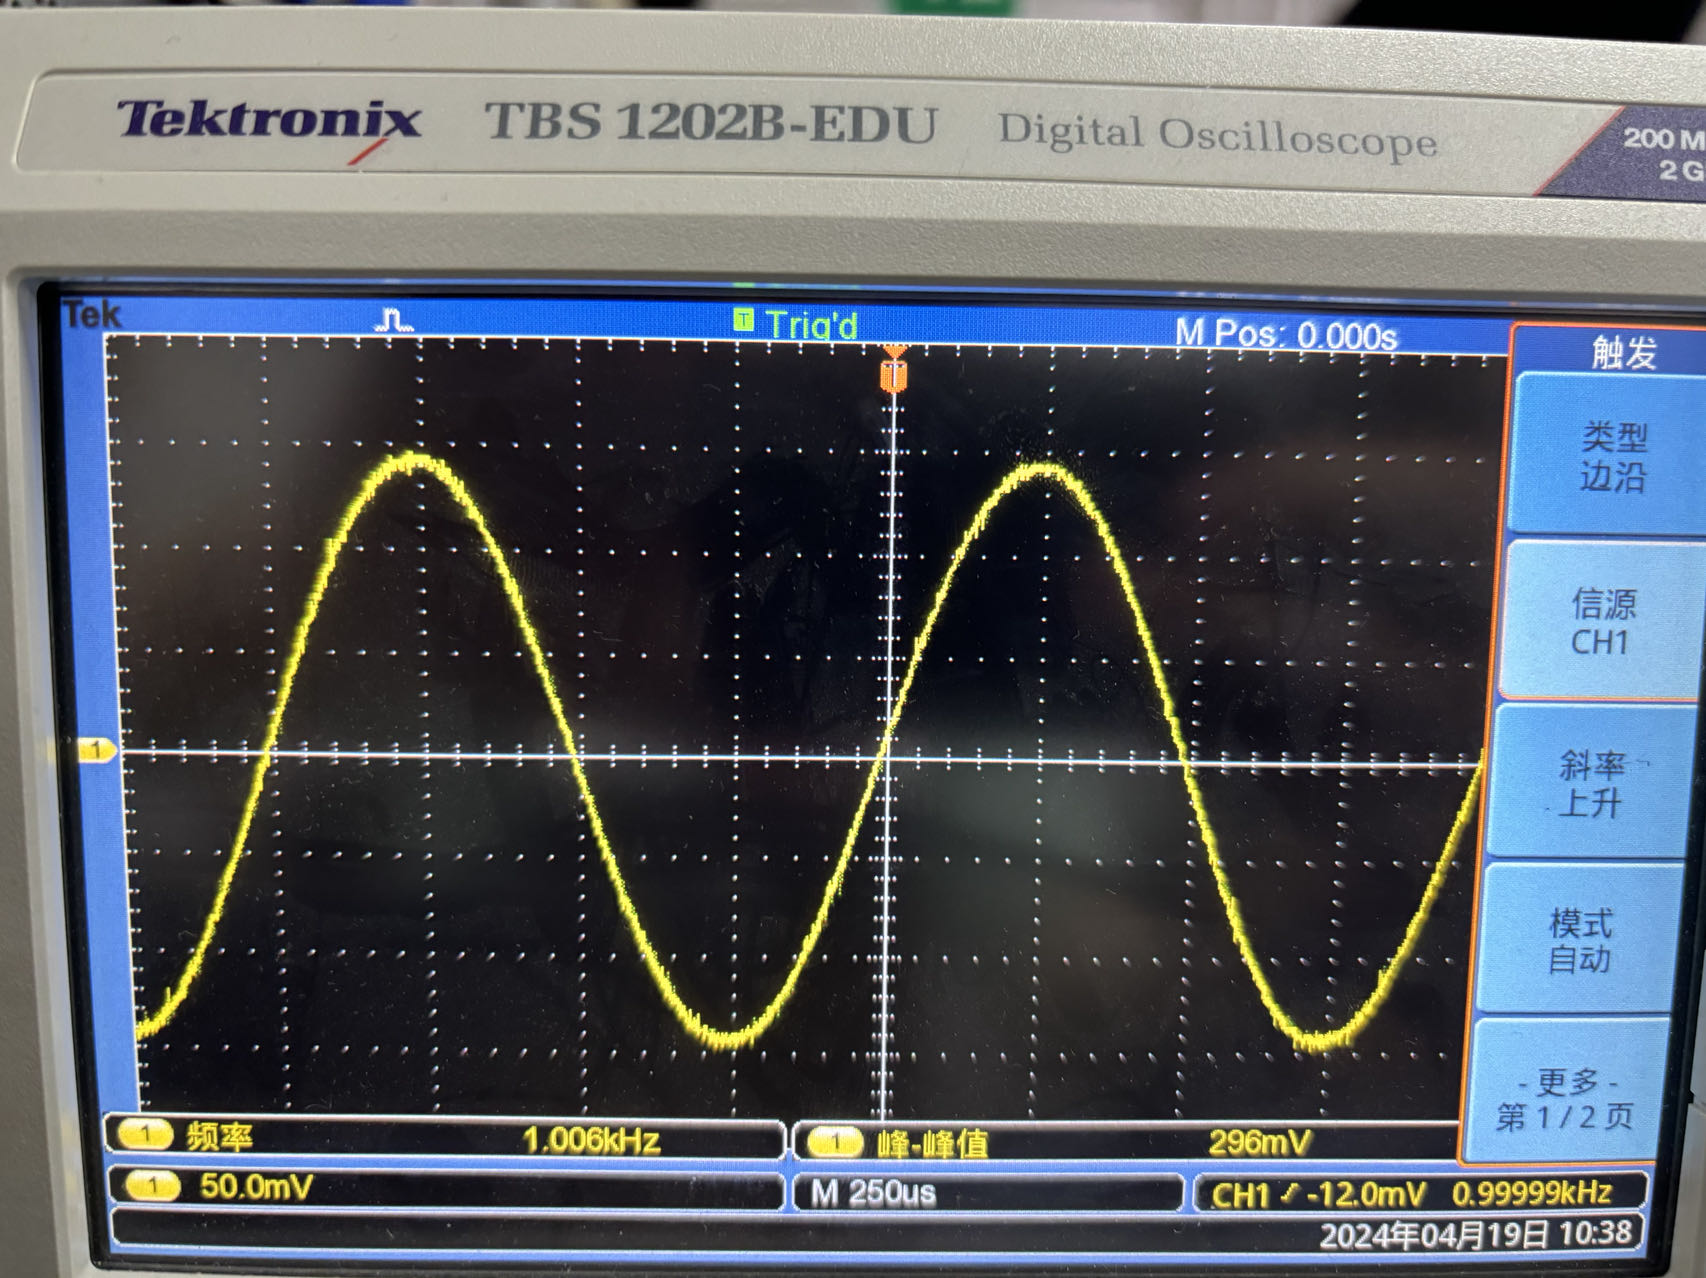
\includegraphics[width=4in]{figure/tri-1kHz.jpg}
  \caption{}
  \label{fig5}
\end{figure}




\end{document}
